\chapter{Sintesi dei materiali}

\section{Sintesi di \emph{quantum dots} di CdSe}
La sintesi di nanocristalli sferici di CdSe è stata eseguita seguendo la procedura messa a punto da Peng \cite{qd-CdSe-CdO}.
Si tratta di una sintesi in micelle inverse
\footnoteremember{micelle-inverse}{{\descriptionlabel{Sintesi in micelle inverse}} sintesi in cui la nanoparticella si forma in una zona polare separata dall'ambiente apolare tramite leganti con code apolari.} 
che utilizza CdO e polvere di selenio. L'utilizzo di micelle inverse\footnoterecall{micelle-inverse} è un metodo di sintesi semplice ed economico che permette un buon controllo della dimensione finale delle particelle e ne impedisce l'aggregazione passivandone la superficie. In letteratura si trovano molte altre procedure di sintesi che differiscono sostanzialmente per le fonti di cadmio e di selenio \cite{qd-CdSe-Cd,qd-CdSe-CdCl2}. Questa via ha come principale vantaggio l'impiego di una sorgente di cadmio non volatile e perciò più sicura rispetto alla migliore alternativa sintetica che comporta l'impiego di dimetilcadmio, volatile, tossico, sensibile all'aria ed esplosivo.

I leganti utilizzati per formare le micelle sono stati tri-{\itshape n}-ottilfosfina ossido (d'ora in poi TOPO) ed acido {\itshape n}-tetradecilfosfonico (d'ora in poi TDPA). Il secondo è un legante di superficie più affine al CdSe rispetto al primo \cite{lig-CdSe-P} ma verrà comunque sostituito nei passaggi di scambio di leganti (Sezione~\ref{sec:leganti}). 

La procedura messa a punto da Peng \cite{qd-CdSe-CdO} prevede di disperdere il CdO nei due leganti e la polvere di selenio in triottilfosfina (d'ora in poi TOP). Dopo aver scaldato e dissolto il CdO vi è stato iniettato rapidamente il Se in TOP\@. Il tutto è stato tenuto a 270°C per 5 minuti. Tutta la procedura è stata svolta in atmosfera di argon e proteggendo il pallone dalla luce. Le nanoparticelle ottenute sono state purificate precipitandole più volte in metanolo disareato per eliminare il TOPO non legato ed il TOP\@. Una volta seccate sotto flusso di azoto sono state ridissolte in toluene e filtrata la soluzione. Le caratterizzazioni effettuate (DLS
\footnoteremember{DLS}{{\descriptionlabel{DLS}} Dynamic Light Scattering, strumento per misurare il diametro idrodinamico di particelle disperse.}
, UV-vis\footnote{La lunghezza d'onda a cui si osserva il primo picco di assorbimento eccitonico può essere utilizzata per determinare il diametro delle NPs di CdSe utilizzando la formula empirica riportata a pagina \pageref{eq:diametro}}
, fotoluminescenza) hanno indicato un diametro di 2.1 - 2.9~nm. La caratterizzazione $^1$H-NMR e $^{31}$P $\{^1H\}$ NMR ha permesso di verificare la presenza dei 2 leganti di superficie.

\section[Sintesi di poli(3-esiltiofene) regioregolare terminato allile/Br]{Sintesi di poli(3-esiltiofene) regioregolare terminato asimmetricamente allile/Br}

La sintesi di poli(3-alchiltiofene) regioregolare può esser effettuata seguendo 3 schemi: metodo McCullough \cite{pol-McCullough}, metodo Rieke \cite{pol-rieke}, Grignard metatesi \cite{pol-grim}. Per quest'ultimo metodo è riportata in letteratura \cite{pol-p3ht-end} la possibilità di sintetizzare un polimero asimmetricamente terminato.
La procedura sintetica seguita per la sintesi di poli(3-esiltiofene) regioregolare terminato asimmetricamente allile/Br è stata sviluppata da Jeffries-El \etal \cite{pol-p3ht-end} e si tratta di una metatesi Grignard. Per questa procedura è riportata in letteratura una cinetica di polimerizzazione quasi vivente \cite{pol-grim-living}. Dato il carattere vivente (discusso più in basso) è possibile ottenere poli(3-esiltiofene) con bassa polidispersità\footnote{{\descriptionlabel{Polidispersità (PDI polydispersity index)}} è una misura della uniformità dei pesi molecolari delle catene polimeriche. Si esprime come rapporto tra la massa molare media pesata e massa media numerica del polimero.}. 

La sintesi avviene in 3 stadi: preparazione del monomero attivo, crescita del polimero, attacco del gruppo di terminazione allile.


\begin{figure}
\centering{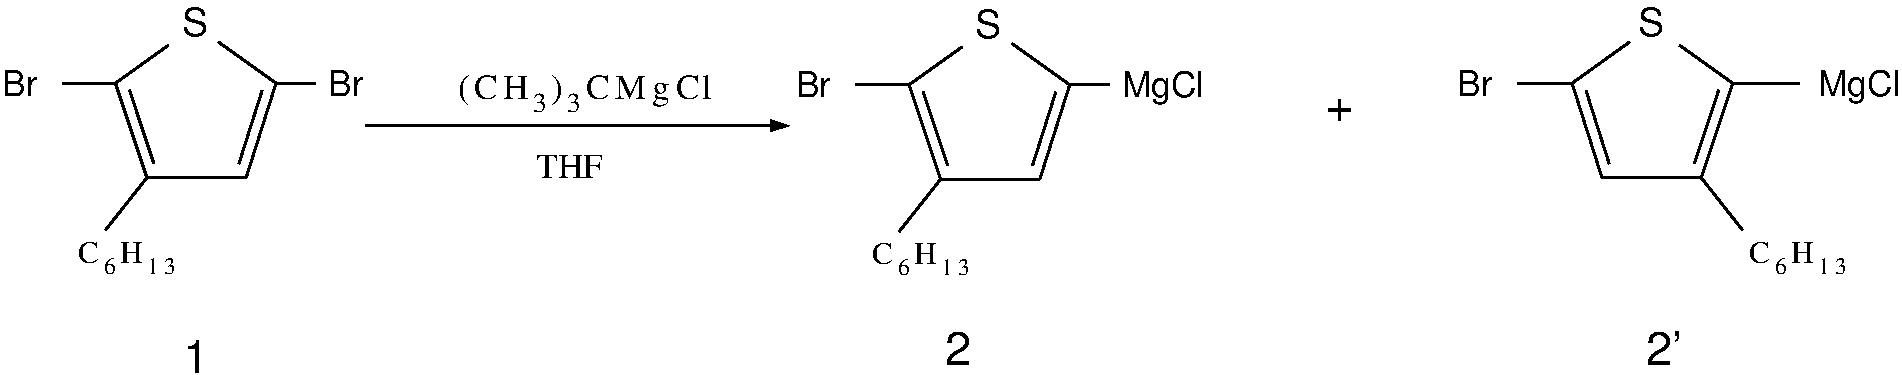
\includegraphics[width=.7\textwidth]{Immagini_Tesi/monomero-grignard.pdf}}
\caption{\footnotesize{Il monomero viene reso un reattivo di Grignard tramite una reazione di metatesi (doppio scambio).}
\label{fig:monomero-grignard}}
\end{figure}
Il monomero 2,5-dibromo-3-esiltiofene è stato trattato con 1 equivalente di \tBu magnesio cloruro e si sono ottenuti i 2 monomeri illustrati in~\ref{fig:monomero-grignard} tramite una reazione di doppio scambio denominata di metatesi Grignard. Nell'articolo di Iovu \etal \cite{pol-grim-living} è riportato il rapporto tra i due prodotti {\bf 2}:{\bf 2'}~=~da~85:15~a~75:25; inoltre nello stesso articolo viene riportato che il prodotto {\bf 2'} non viene consumato dalla polimerizzazione.

Successivamente è stato aggiunto il catalizzatore a base di Nickel: 1,3-bis(difenilfosfino) propano nickel(II) cloruro per avviare la polimerizzazione. 
Uno dei meccanismi proposti è illustrato in~\ref{fig:pol-polimerizz}.
\begin{figure}
\centering{
\includegraphics[width=.8\textwidth]{Immagini_Tesi/pol-polimerizz.png}}
\caption{\footnotesize{Il meccanismo proposto per la polimerizzazione GRIM del poli(3-alchiltiofene). Immagine tratta da \cite{pol-grim-living}.}
\label{fig:pol-polimerizz}}
\end{figure}
Il primo stadio consiste nello scambio tra i due anioni \ce{Cl-} e due formali anioni derivanti dal Grignard del monomero. Quindi con una eliminazione riduttiva si ha la formazione di un dimero \emph{tail-tail}\label{tail-tail}. Dopo la formazione del dimero il catalizzatore vi resta legato in una coppia associata da cui poi ha il via la polimerizzazione vera e propria. 
Lo stadio lento del ciclo di polimerizzazione, che causa il carattere quasi vivente, è la transmetallazione. 

Infine, come illustrato in~\ref{fig:grim-end}, si è aggiunto allilmagnesio bromuro per terminare un solo capo della catena polimerica con un gruppo allile. Non avviene il doppio attacco ad entrambe le terminazioni perché si ha formazione di una coppia associata tra il catalizzatore ed il primo gruppo terminante inserito. Nell'articolo \cite{pol-p3ht-end} da cui è tratta questa procedura vengono riportati anche altri reattivi di Grignard con cui è possibile ottenere una singola terminazione. Alcuni di questi reattivi sono stati testati in precedenti lavori del nostro gruppo e la migliore resa è stata ottenuta utilizzando allilmagnesio bromuro.

\begin{figure}
\centering{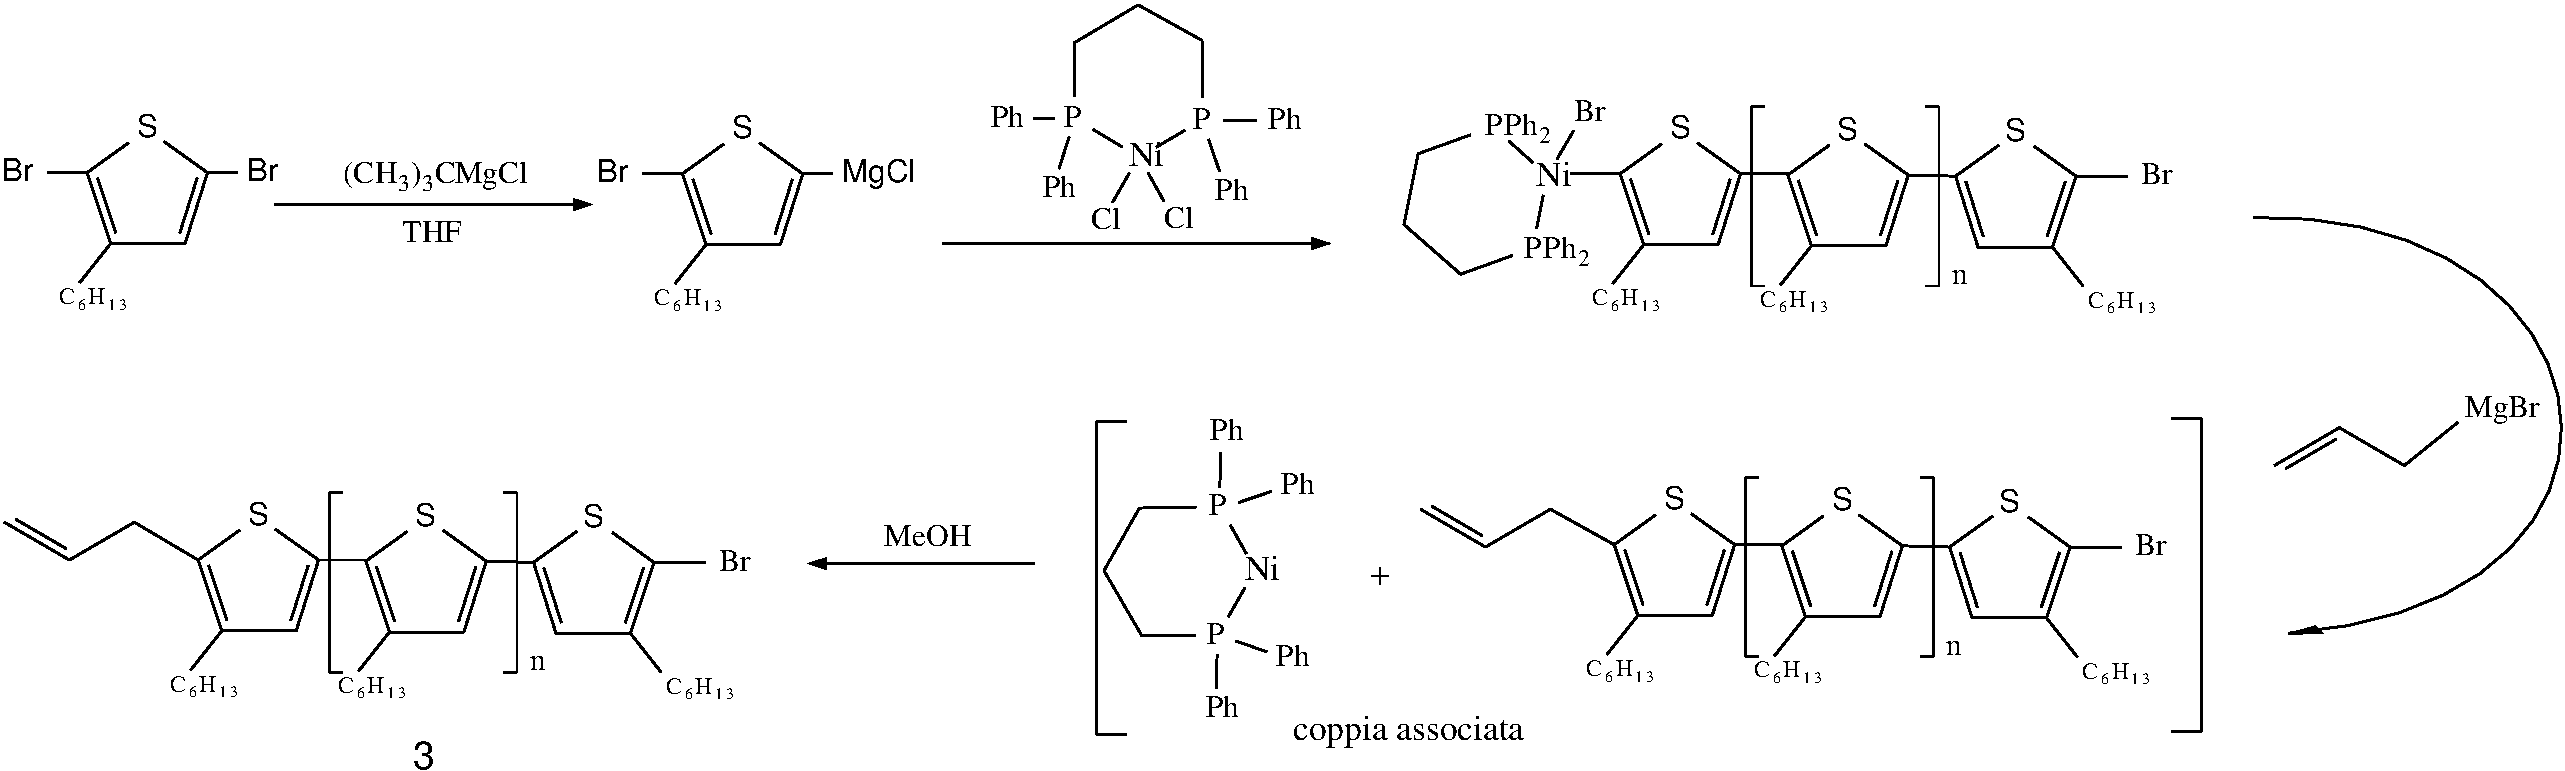
\includegraphics[width=.99\textwidth]{Immagini_Tesi/grim-end.pdf}}
\caption{\footnotesize{Lo schema generale della polimerizzazione e della terminazione.}
\label{fig:grim-end}}
\end{figure}
Il prodotto {\bf 3} è stato purificato con metanolo e {\itshape n}-esano ed infine raccolto in cloroformio e seccato. 

La caratterizzazione $^1$H-NMR ha permesso di verificare la regioregolarità, la terminazione asimmetrica e di stimare la lunghezza del polimero.
\section{Sintesi di poli(3-esiltiofene) terminato allile/legante fosfonico}
In questa sezione si espone la modifica del prodotto \n{3} della sezione precedente al fine di ottenere un gruppo legante su una delle due terminazioni del polimero. L'attacco avverrà sulla terminazione presentante un bromo sfruttando la sua reattività in un \emph{coupling} di Sonogashira. Invece la terminazione allilica resterà inalterata e presente sul polimero finale \n{7}.

 Si ha a disposizione la molecola dietil (4-bromofenil)fosfonato ({\bf 4}) precedentemente sintetizzata che presenta un gruppo fosfonico protetto da etili. 

La sintesi si può dividere in 3 fasi: modifica del legante ed attacco al polimero entrambi con un \emph{coupling} di Sonogashira ed infine deprotezione del gruppo fosfonico.

Come illustrato in~\ref{fig:legante} al legante è stato aggiunto tramite un \emph{coupling} di Sonogashira un gruppo alchinico monoprotetto con il gruppo trimetilsilile per non dare ulteriore accoppiamento. 
\begin{figure}
\centering{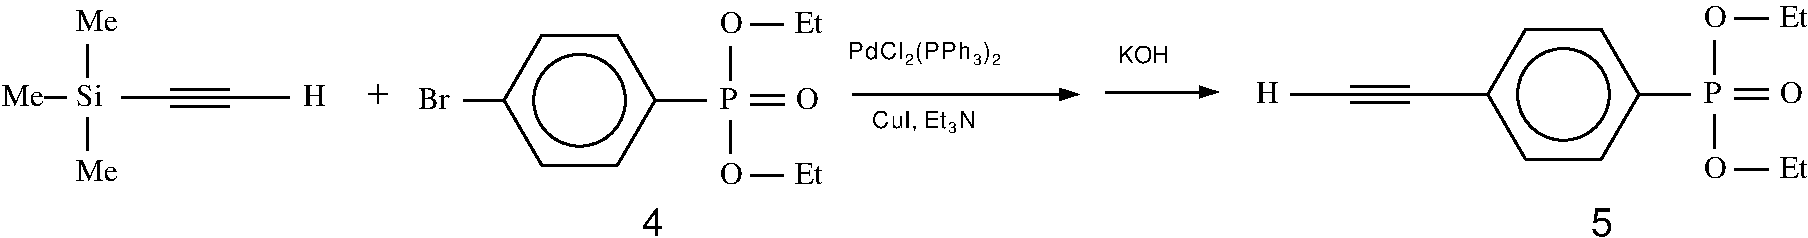
\includegraphics[width=1\textwidth]{Immagini_Tesi/legante.pdf}}
\caption{\footnotesize{Schema della modifica e della deprotezione del legante.}
\label{fig:legante}}
\end{figure}

Quindi la protezione è stata rimossa con KOH e, dopo purificazione su colonna, è stato eseguito un secondo \emph{coupling} di Sonogashira tra il legante \n{5} ed il polimero \n{3} terminato allile/bromo come illustrato in~\ref{fig:p3ht-legante}. Infine è stata rimossa la protezione del gruppo fosfonico utilizzando trimetilbromosilano per ottenere il polimero finale \n{7}. 
\begin{figure}
\centering{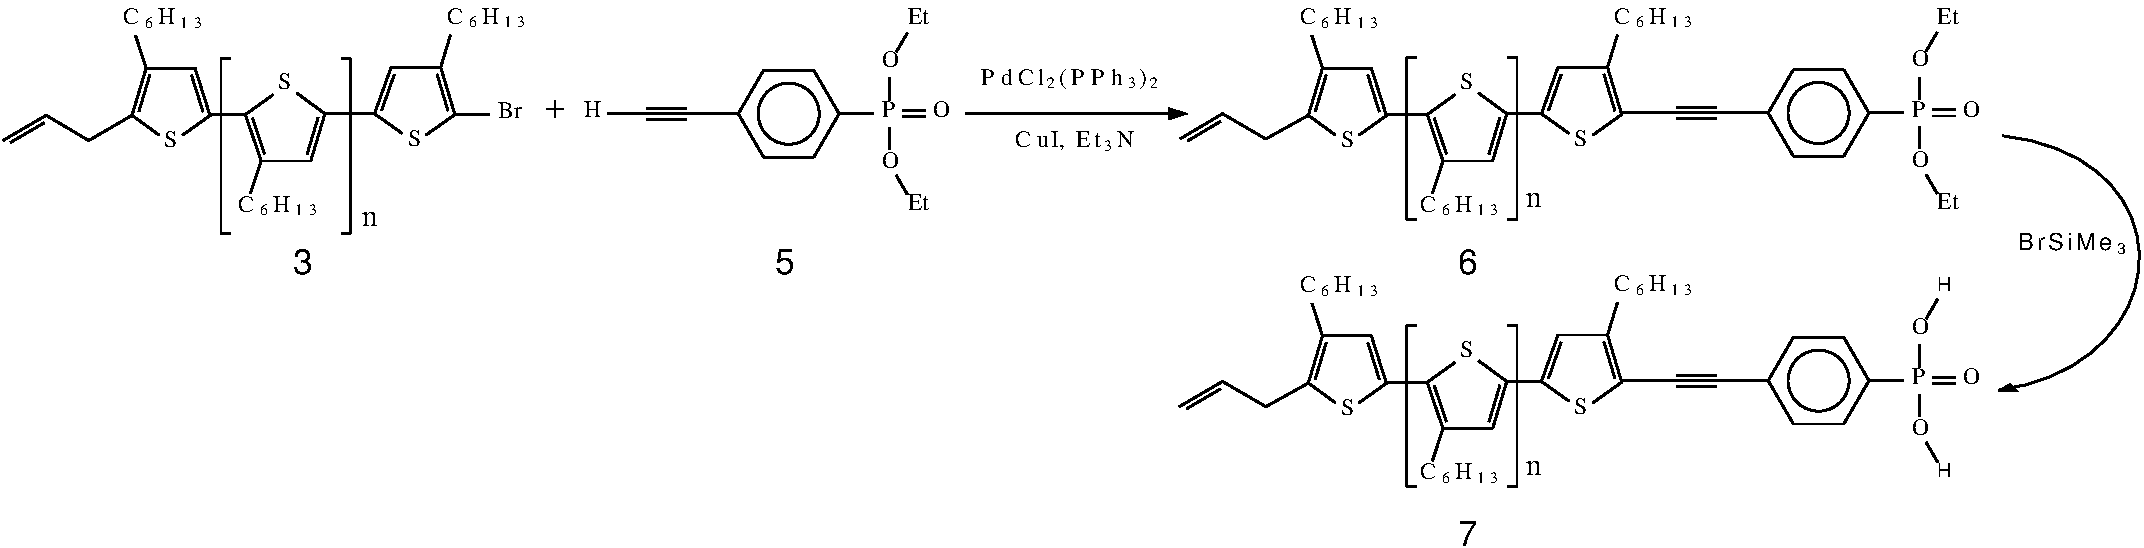
\includegraphics[width=1.1\textwidth]{Immagini_Tesi/p3ht-legante.pdf}}
\caption{\footnotesize{Schema del \emph{coupling} di Sonogashira tra il legante \n{5} ed il polimero \n{3} con successiva deprotezione a \n{7}.}
\label{fig:p3ht-legante}}
\end{figure}

La caratterizzazione $^1$H-NMR del polimero finale, costituito da una catena oligomerica idrofoba con una 
terminazione idrofila, non ha consentito di evidenziare la presenza dei segnali relativi alla terminazione legante. Questo fatto inatteso si ritiene sia dovuto non alla mancata funzionalizzazione ma piuttosto alla formazione di strutture micellari, cioè di sistemi quasi solidi non analizzabili con tecniche convenzionali di NMR in soluzione~\cite{lig-micelle-nmr2}. 

\section{Scambio di leganti}
\label{sec:leganti}
Allo scopo di ottenere i \emph{quantum dots} passivati almeno in parte dal polimero sintetizzato \n{7} è necessario effettuare uno scambio di leganti di superficie. Purtroppo il gruppo legante presente su {\bf 7} ha una affinità per la superficie delle NPs comparabile con l'affinità del TOPO e del TDPA\@. Dunque uno scambio diretto avrebbe una resa limitata. È possibile ovviare a questo problema effettuando due scambi di leganti: la sostituzione di TOPO con un legante blando come la piridina e successivamente lo scambio della piridina col polimero \n{7}.

 Si prevede che la maggior parte del TOPO (una trialchil fosfina ossido) venga sostituito dalla piridina, mentre il TDPA (un acido fosfonico) essendo più affine alla superficie \cite{lig-CdSe-P} dovrebbe esser rimosso più difficilmente. 
Questo primo scambio di leganti viene eseguito semplicemente sciogliendo le NPs in piridina e scaldando per tempo sufficiente. La procedura è stata sviluppata da Peng \etal \cite{lig-pyridine}. Le nuove nanoparticelle parzialmente passivate con piridina sono risultate, al contrario di quelle stabilizzate solo dai leganti fosforati aventi lunghe catene alchiliche, solubili in metanolo ed insolubili in {\itshape n}-esano. La procedura di sostituzione e purificazione è consistita in diversi cicli di dissoluzione in piridina e precipitazione in {\itshape n}-esano.

Nel secondo scambio, in cui si vuole ottenere le NPs di CdSe passivate col polimero {\bf 7}, è necessario utilizzare un solvente che solvati entrambi i precursori, ossia sia le particelle passivate con TOPO, TDPA e piridina che il politiofene con funzionalità terminale fosfonica, come tetraidrofurano o cloroformio. Si è scelto di utilizzare come solvente il cloroformio, quindi vi sono stati disciolti uguali pesi di polimero e di \emph{quantum dots} e si è lasciato procedere lo scambio di leganti a temperatura ambiente. Il rapporto in peso di polimero e nanoparticella è stato scelto sulla base delle indicazioni di letteratura scientifica relative ai sistemi oggetto di studio in grado di dare l'efficienza energetica più elevata~\cite{qd-ratio-CdSe_vs_pol}.


